\documentclass[a4paper,11pt]{article}

\usepackage{graphicx}
\usepackage{subfig}


\begin{document}
\title{ML CS726 Fall'11 Project 1 Basic Classifiers}
\author{Angjoo Kanazawa, Ran Liu, Austin Myers}
\maketitle


\section{Writeup}
\subsection{Warm up}
\textbf{WU1}:\textsf{Why is this computation equivalent to computing classification
accuracy?}\\

This computation is equivalent to computing classification accuracy
because it first compares the ground truth classifications with the
predictions, and where they are equal this operation yields ones, otherwise
zeros. The mean of this array is the number of ones, correct classifcations, divided by the
total, which is equivalent to classification accuracy.

\subsection{Decision Tree}
\textbf{WU2}:\textsf{ We should see training accuracy (roughly) going down and
test accuracy (roughly) going up.  Why does training accuracy tend to
go down?  Why is test accuracy not monotonically
increasing?}\\

Training accuracy tends to go down because we're training the
algorithm on that data with answers. The design of the tree is s.t. we
minimize the training error. However the test accuracy is not
monotonically increasing because there may be examples that the
algorithm is not ready for. In another words the more the accuracy
goes up on the training set the more algorithm will over-fit on that
specific training set and thus not generalize well to the unseen test set.\\

\noindent
\textbf{WU3:} \textsf{You should see training accuracy monotonically increasing
and test accuracy making a (wavy) hill.  Which of these
is guaranteed to happen a which is just something we might
expect to happen?  Why?}\\

We can guarantee that the training accuracy will monotonically
increase. This is because the deeper we go, the better our tree will
fit the training data. By construction when the tree is complete as
long as the training set is consistent we will have 0 error. We should
expect the test set to make a wavy hill because we can't guarantee that
our training set is representative of the test set, or the entire
distribution datasets are taken from. So if we overfit it will go up,
but we might focus on the right feature, or hope to do so, to increase
the accuracy on the test set. But we can never guarantee that the
accuracy of the test set will monotonically increase.\\

\noindent
\textbf{WU4}: \textsf{Train a decision tree on the CG data with a maximum depth
of 3.  If you look in \texttt{datasets.CFTookCG.courseIds}
and \texttt{courseNames} you'll find the corresponding course for
each feature.  The first feature is a constant-one "bias" feature.
Draw out the decision tree for this classifier, but put in the actual
course names/ids as the features.  Interpret this tree: do these
courses seem like they are actually indicative of whether someone
might take CG?}
The decision tree trained on the CG data with maximum depth 3 looks
like:
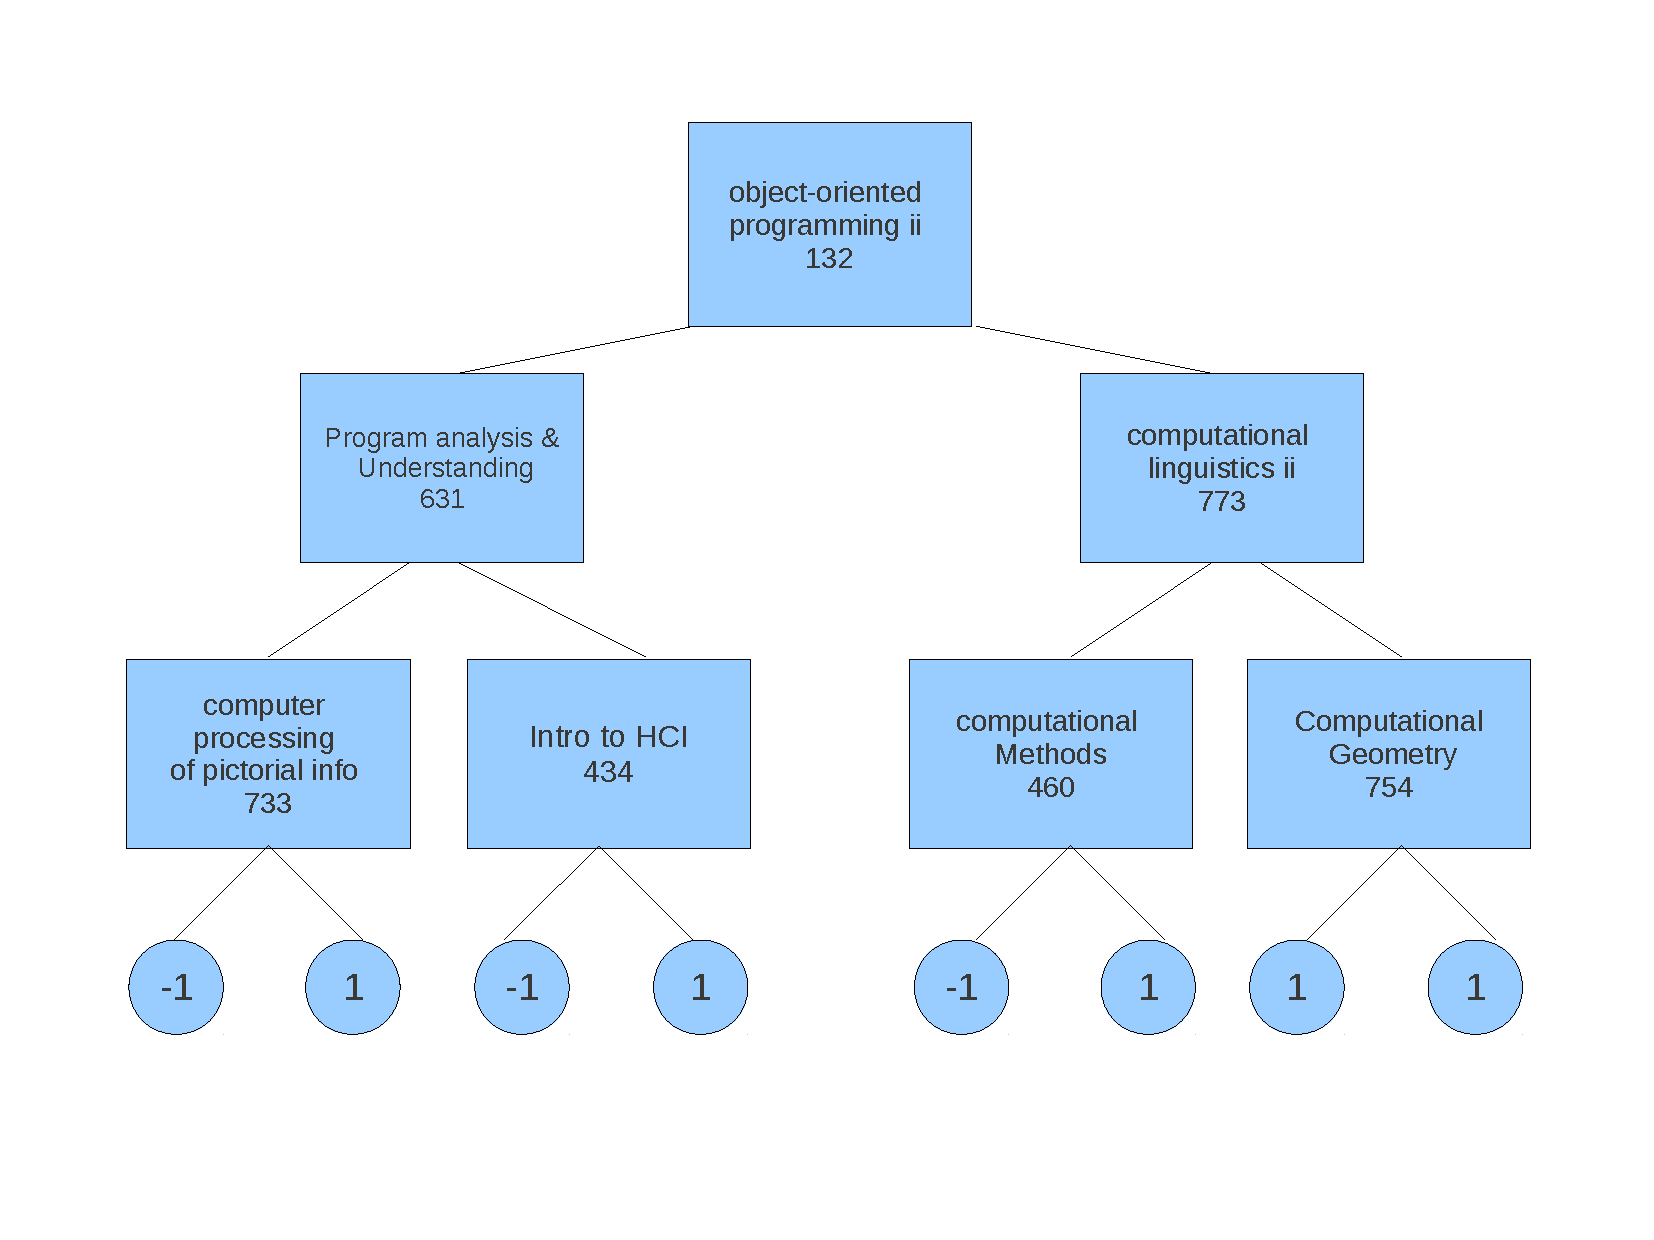
\includegraphics[width=5in]{DTdrawing.pdf}
Most of the  features do seem like they would positively correlate
with a student who has taken CG. According to the decision tree,
students who have taken
Computational Geometry, Pictorial Information and Computational
Methods, and HCI are more likely to have taken CG. These courses are
graduate courses which a student who is in graphics, geometry, or
vision would take.

\subsection{KNN}
\textbf{WU5:} \textsf{For the course recommender data, generate train/test
curves for varying values of K and epsilon (you figure out what are
good ranges, this time).  Include those curves: do you see evidence of
overfitting and underfitting?  Next, using K=5, generate learning
curves for this data.}
 
For epsilon ball (figure 1),  we can see clearly see overfitting. When epsilon is
less than 3.5, the training accuracy is super high and the accuracy on
test data is very low (lower than 0.5). Clearly it's been
overfitted. When eps is greater than 6, it's underfitting because
both the training and test accuracy are low. At this point epsilon is
merely taking the average of all data points and thus underfitting. 

For KNN (figure 2), when k=1, it's overfitting, the test accuracy is perfect while the testing accuracy
is only 0.5. There is no clear sign of underfitting there, but when k
gets bigger (k=8,9,10), from figure 2 we can see the training
accuracy is going lower and lower and the testing accuracy is getting
lower as well. That is an indication of underfitting.\\
The learning curve for KNN with K=5 is figure 3.
\begin{figure}[h!]
  \caption{epsilon on varying values of eps}
 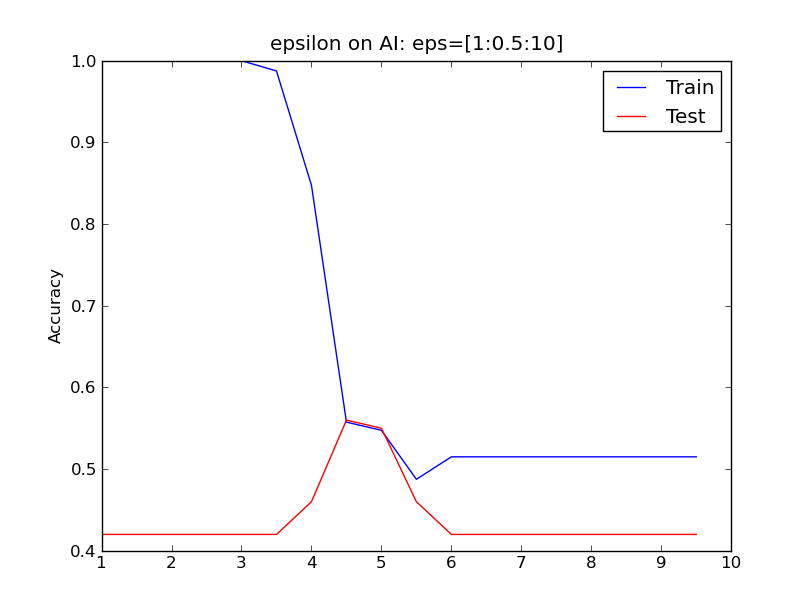
\includegraphics[scale=0.5]{epsOnAi_hyper.png}
\end{figure}
\begin{figure}[h!]
  \caption{KNN on varying values of K}
   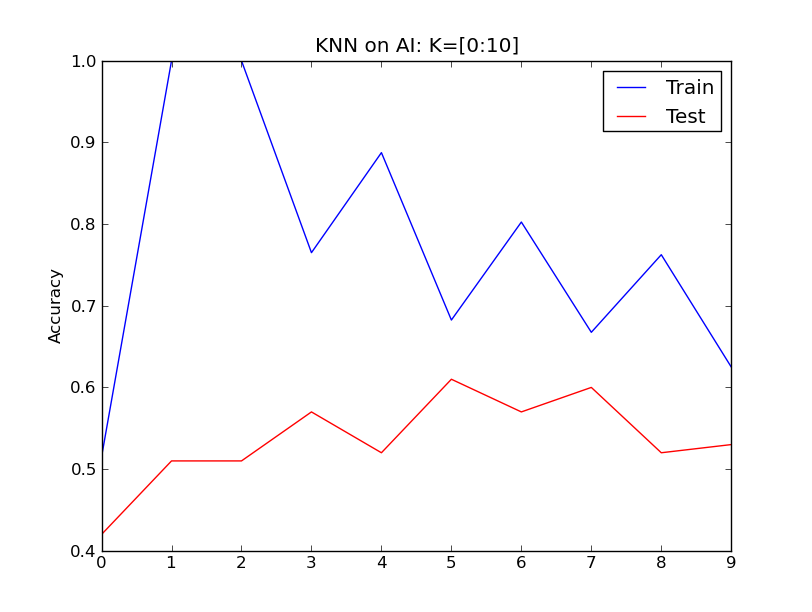
\includegraphics[scale=0.5]{knnOnAi_hyper.png}
\end{figure}
\begin{figure}[h!]
  \caption{Learning curve of KNN with K=5}
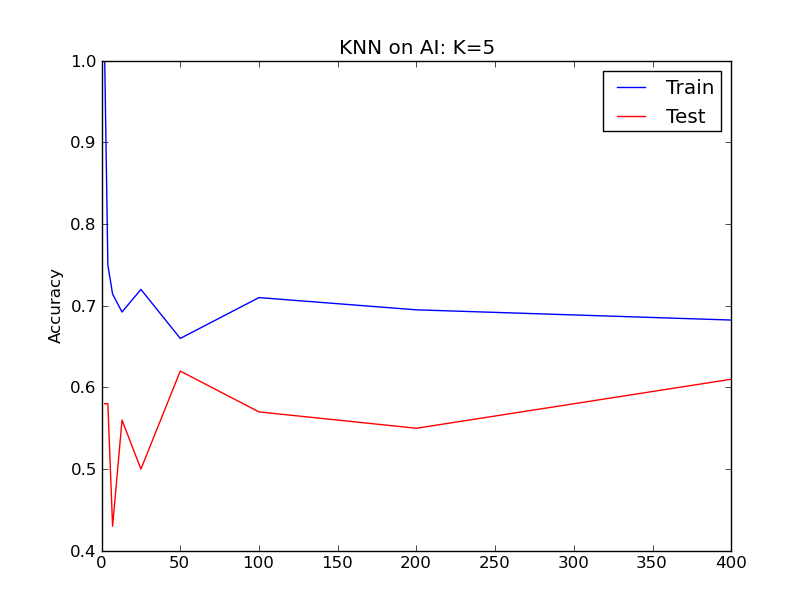
\includegraphics[scale=0.5]{knnOnAI.png} 
\end{figure}


\pagebreak
\pagebreak
\subsection{Perceptron}
\textbf{WU6:} \textsf{Take the best perceptron you've been able to find
  so far on the AI data.  Look at the top five positive weights (those
  with highest value) and top five negative weights (those with lowest
  value).  Which features do these correspond to?  Can you explain why
  these might get these features as the "most indicative"?  Why is it
  hard to interpret "large weight" as "most indicative"?  How do these
  large weighted features compare to the features selected by the
  decision tree?}\\


The features corresponding to the top 5 positive weight were:

\begin{enumerate}
\item (weight: 9) 'computer processing of pictorial information' 
\item (weight: 8) 'advanced computer graphics'
\item (weight: 7) 'database management systems'
\item (weight: 5) 'data structures'
\item (weight: 5) 'introduction to information technology' (also
  weight 5 are 'computer networks (417)','computational methods')

\end{enumerate}
The features corresponding to the top 5 negative weights were:

\begin{enumerate}
\item (weight: -8) 'honors seminar'
\item (weight: -6) 'introduction to c programming'
\item  (weight: -5) 'program analysis and understanding'
\item (weight: -5) 'object-oriented programming i'
\item (weight: -4) 'computer networks (711)', 'bias',   'introduction to human-computer interaction' 
\end{enumerate}

The 5 most negative weights include a non-CS
major class, a 200-level 1 credit Pass/Fail course, and an
introductory course 131. This is likely
because in the first case non-CS majors will not take 421 and in the
case of the other two courses some of the students just starting in CS
may not continue in the program long enough to take 421. The 5 most positive
courses are mostly graduate level courses, which makes it more likely
that they have taken AI.

It is difficult to interpret large weights as ``most indicative'' because there may exist a group of more indicative
features which have distributed weights among themselves.\\

The top 4 levels of the decision tree contain the 4 most positive weights
from the perceptron ('databse management, 'introduction to information
technology','advanced computer graphics', 'computer processing of
pictorial information') where the decision tree's prediction agrees 
with the perceptron. However, there are numerous courses used in the 
decision tree that do not appear in the most positive and negative weights. 
      
\end{document}
